\documentclass[11pt]{article}
\usepackage[margin=0.7in]{geometry}
\newcommand{\ts}{\textsuperscript}
%Gummi|065|=)
\date{}
\usepackage{caption}
\usepackage{subcaption,graphicx}
\usepackage{lineno, blindtext}
\usepackage{color}
\usepackage{graphicx}
\usepackage{hyperref}
\hypersetup{
    colorlinks=true,
    linkcolor=blue,
    filecolor=magenta,      
    urlcolor=cyan,
    pdftitle={Sharelatex Example},
    bookmarks=true,
    pdfpagemode=FullScreen,
}
\urlstyle{same}

\title{Table of Contents}

\begin{document}
\maketitle

\tableofcontents

\newpage

\listoffigures

\newpage

%%%%%%%%%%%%%%%%%%%%%%%%%%%%%%%%%%%%%%%%%%%%%%%%%%%%%%%%%%%%%%
%%															%%
%% 							Section 1    					%%
%% 															%%
%%%%%%%%%%%%%%%%%%%%%%%%%%%%%%%%%%%%%%%%%%%%%%%%%%%%%%%%%%%%%%

\section{Progress Report}
\subsection{1\ts{st} Iteration}
Should be achieved by: July 12, 2016
\begin{itemize}
\item Robot moves forward exactly one cell length and turns 90 $^{\circ}$ accurately\\
This is the most important feature of our robot. By ensuring accurate movement, we limit the need to readjust in each cell.
\item Robot follows right wall\\
This is the algorithm needed to find the unique solution to the maze. Once movement is implemented, we can just build on top of it to collect more data as we move through the maze. 
\end{itemize}

\subsection{2\ts{nd} Iteration}
Should be achieved by: July 12, 2016
\begin{itemize}
\item Robot tracks its orientation and location in maze\\
This is a dependency for most of the other requirements. By tracking movement in the maze, we are able to know when we have reached our goal, how we reached it (in order to implement coming back shortest path) and where to store cell information in our 2-D array.
\item Robot beeps when it has reached the target cell
\item Robot stores wall information, visited/unvisited status and orientation at entry in a 2-D array.\\
This is required for more advanced algorithm features we wish to implement such as having the robot not check the same wall twice. Furthermore, this was required in order to display current location and wall information graphically. We chose to implement it now because it was a major criteria requirement. 
\end{itemize}

\subsection{3\ts{rd} Iteration}
Should be achieved by: July 19, 2016
\begin{itemize}
\item Robot returns with the shortest path\\
Since we know the route we took to get to our final location, we can now implement the canceling algorithm (described in detail in \textbf{Subsection 3.16}).
\item Robot displays current location graphically on screen\\
We are implementing this now, so that we could test our algorithm more easily. The last project feature we wanted to implement was to not check the same wall twice. This would be difficult to implement without sufficient debugging capabilities. As such, we improved our debugging capabilities before continuing.
\end{itemize}

\subsection{4\ts{th} Iteration}
Should be achieved by: July 26, 2016
\begin{itemize}
\item Improve algorithm such that robot does not check same wall twice\\
Suppose the robot is in a cell with a wall to the South. If we've checked that there is a wall toward the South, the robot should store the fact that in the cell below our current cell, there is a wall to the North and act accordingly. In this case, the robot should not check North wall when it is in the cell below the current cell. The most general case will be programmed and described in \textbf{Section 3}. This has two major advantages: the robot does not waste time turning and the robot does not incur extra error because of unnecessary turning.
\end{itemize}
\newpage


%%%%%%%%%%%%%%%%%%%%%%%%%%%%%%%%%%%%%%%%%%%%%%%%%%%%%%%%%%%%%%
%%															%%
%% 							Section 2    					%%
%% 															%%
%%%%%%%%%%%%%%%%%%%%%%%%%%%%%%%%%%%%%%%%%%%%%%%%%%%%%%%%%%%%%%


\section{Mechanical Design of MazeBot}
\subsection{Top Level Mechanical Structure and Specifications}
Our robot needed to have very accurate movement in order to be successful in the maze. This specification depends heavily on whether or not the motor encoders report accurate values to the algorithm. In order to have the motor encoders reporting accurrately, we had to ensure:
\begin{itemize}
\item The wheels do not slip
\item The robot does not hit walls
\item The drive system is sturdy 
\item The gears are securely held in place and make proper contact. 
\end{itemize}
However, there is a limit to how much we can minimize mechanical error in movement. As a result, we will have to readjust after a certain number of cells (\textbf{Subsection 3.16}). However, having to readjust too often is problematic as this increases average time in each cell which is a major criteria point. As a result, we hope to minimize how often we need to readjust by maximizing the accuracy of the mechanical system. 
\newpage

\subsection{First Iteration}

\begin{itemize}
\item \textbf{Goals:}
	\begin{itemize}
	\item Able to go 3 cells without needing to readjust
	\item Able to turn 90$^{\circ}$ accurately.
	\end{itemize}
\end{itemize}
\begin{figure}[htp]
\centering
\captionsetup{justification=centering}
\minipage{0.32\textwidth}
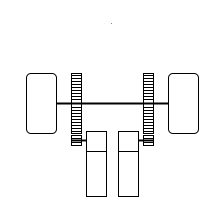
\includegraphics[scale=0.80]{images/Hardware_Mechanical/First_Iteration_Design_Driving_System.png}
\caption{First Iteration Drive System}\label{fig:Drive System}
\endminipage\hfill
\minipage{0.32\textwidth}
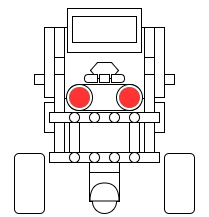
\includegraphics[scale=0.79]{images/Hardware_Mechanical/First_Iteration_Design_FrontView.png}
\caption{First Iteration Front View}\label{fig:Front View}
\endminipage\hfill
\minipage{0.32\textwidth}
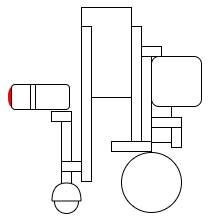
\includegraphics[scale=0.79]{images/Hardware_Mechanical/First_Iteration_Design_SideView.png}
\caption{First Iteration Side View}\label{Side View}
\endminipage
\end{figure}
\begin{figure}[!tbp]
  \centering
  \begin{minipage}[b]{0.34\textwidth}
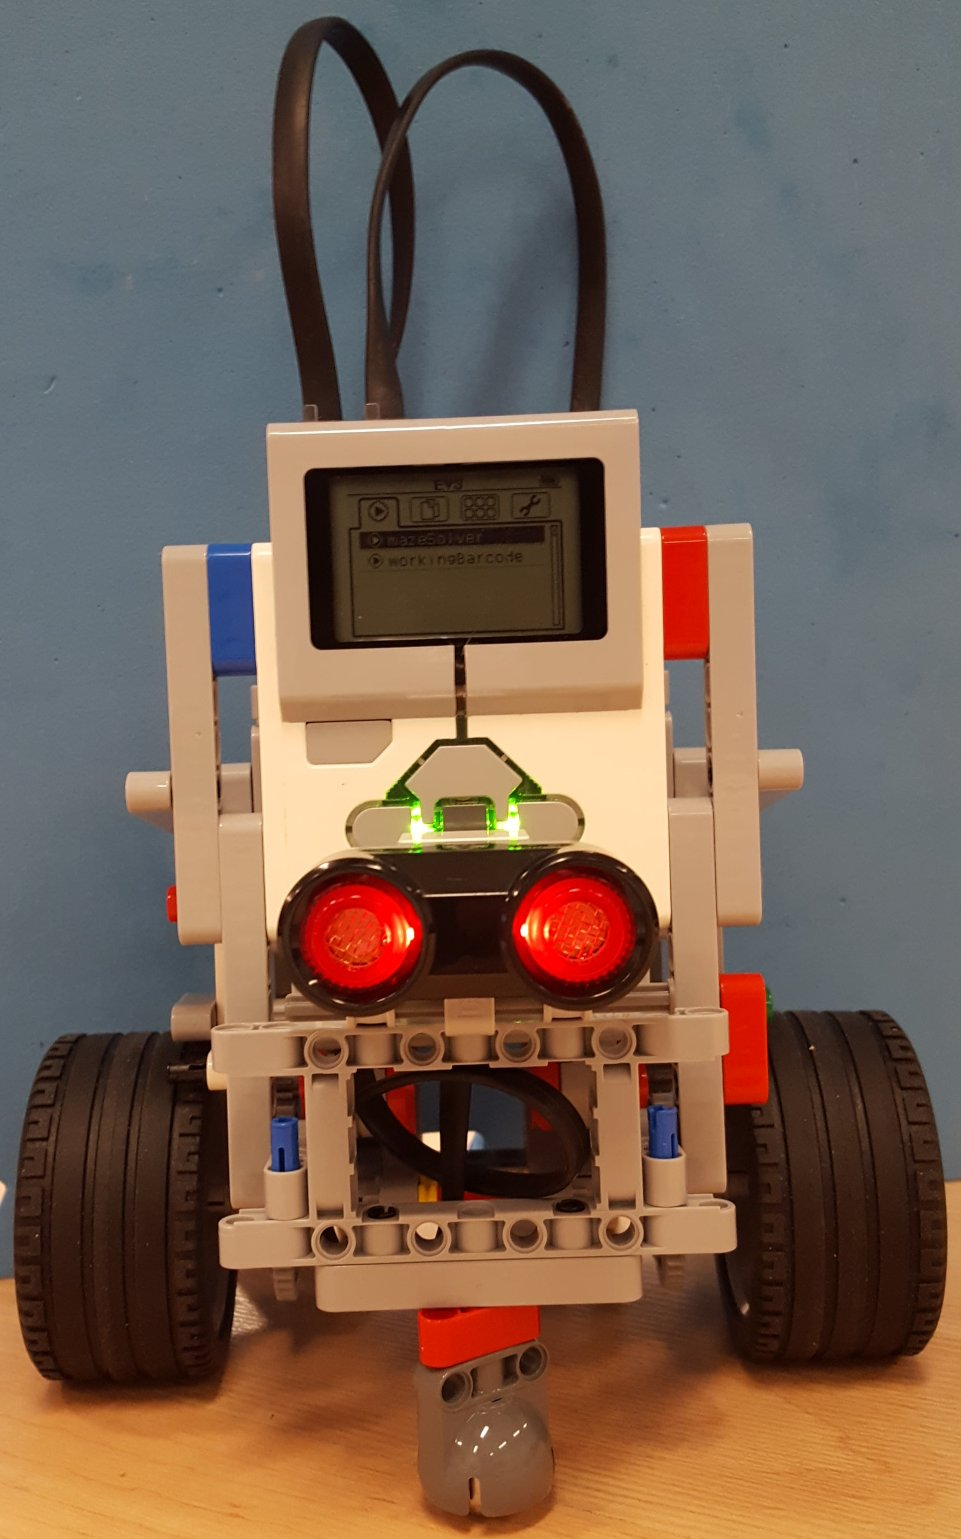
\includegraphics[scale=0.18]{images/Hardware_Mechanical/First_Iteration_Front.jpg}
\caption{First Iteration Front View}\label{fig:Front View}
  \end{minipage}
  \hfill
  \begin{minipage}[b]{0.4\textwidth}
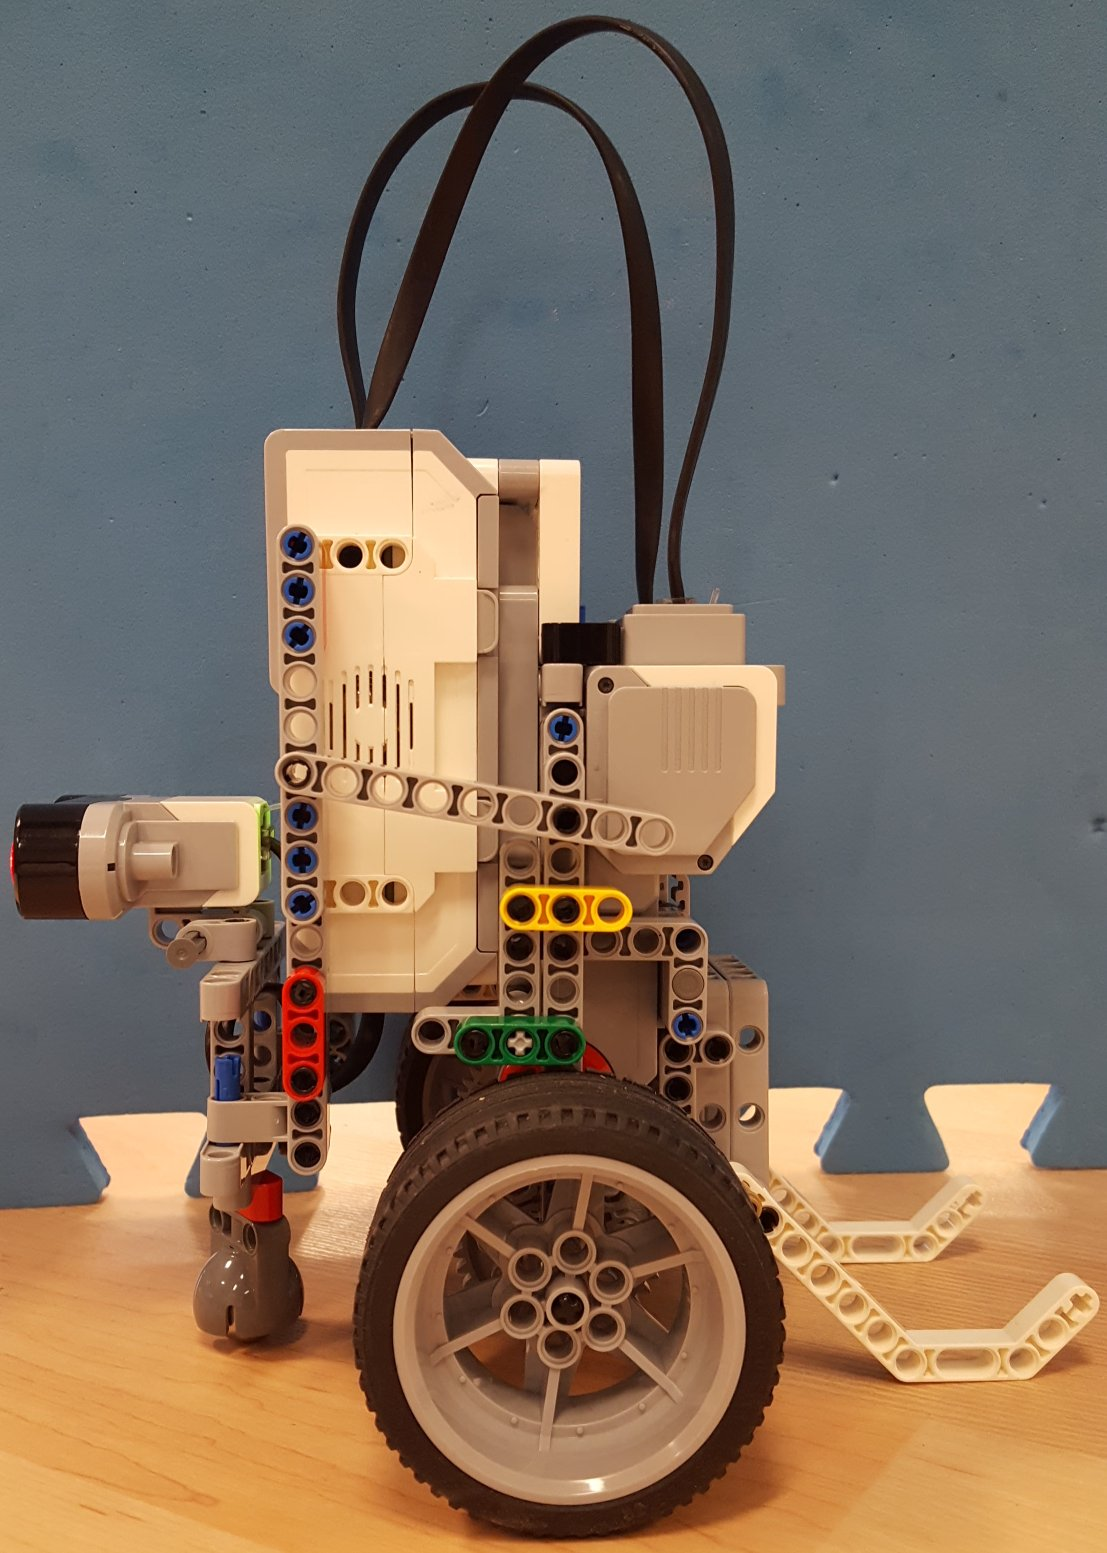
\includegraphics[scale=0.18]{images/Hardware_Mechanical/First_Iteration_Left.jpg}
\caption{First Iteration Side View}\label{Side View}
  \end{minipage}
\end{figure}
\newpage
\begin{itemize}
\item \textbf{Observations \& Measurements}
	\begin{itemize}
	\item \textbf{Goal}: Robot is able to go 3 cells without needing to readjust
	\item \textbf{Failed}: Robot needed to readjust every second cell
	\item \textbf{Goal}: Robot is able to turn 90$^{\circ}$ accurately.\\
	Test - An error of even $ \pm 1^{\circ}$ will accumulate to a significant error when traversing cells. However, error in a single turn is hard to notice. Therefore, we chose to have the robot turn 90$^{\circ}$ 8 times in place in order to propagate any error significantly.
	\item \textbf{Failed}: Robot had error of $ \pm 24^{\circ}$
	\end{itemize}
\item \textbf{Reasons for Test Failures}
	\begin{itemize}
	\item \textbf{Structural Integrity of the Drive System}\\
	We were unable to find space to properly secure the left and right drive wheels. When testing, we found one wheel slipped forward and the other wheel slipped back when turning. This problem defeated the accuracy of the encoder. Hence, we were unable to meet our goal of accurate movement.
	\item \textbf{Robot is too Large.}\\
	Since the brick is upright, the robot is top heavy. We needed two white bars in the back and one metal ball in the front to balance the robot. The additions of the two white bars and one metal ball negates the spacial advantage of having the robot's brick be upright. Even though the dimensions of the robot were within the size of one cell, it left very little room for movement error. As such, the robot began to run into walls after the second turn.
	\item \textbf{Wheels are too Big}\\
	In order for the motor encoder to be accurate, the wheels must not slip. Therefore, to maximize friction, we decided to use the largest wheels in the brickset. However. the extra friction with the ground from the larger wheels is not worth the extra size added to the robot. When we replaced the large wheels with smaller wheels, we noticed little to no change in accuracy of movement.
	\end{itemize}
\item \textbf{Conclusion}\\
In conclusion, we have decided to not have the brick upright. This will allow us to have enough room to properly secure the drive system. As such, the gears will make proper contact and will not slide forward or backward. This ensures maximum encoder accuracy. By having the robot level with the table, we will be able to take out the additional support that we needed before to hold the bot upright. Similarily, we chose to use wheel with smaller radius but same thickness. Both of these changes will allow more room for movement error when turning and going into new cells.
\end{itemize}
\newpage

\subsection{Second Iteration}
\begin{itemize}
\item \textbf{Goals:}
	\begin{itemize}
	\item Able to go 3 cells without needing to readjust
	\item Able to turn 90$^{\circ}$ accurately.
	\end{itemize}
\end{itemize}
\begin{figure}[htp]
\centering
\captionsetup{justification=centering}
\minipage{0.32\textwidth}
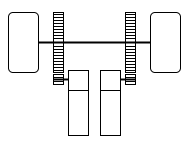
\includegraphics[scale=0.80]{images/Hardware_Mechanical/Third_Iteration_Design_drive.png}
\caption{Second Iteration Drive System}\label{fig:Drive System}
\endminipage\hfill
\minipage{0.32\textwidth}
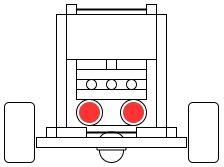
\includegraphics[scale=0.70]{images/Hardware_Mechanical/Third_Iteration_Design_front.png}
\caption{Second Iteration Front View}\label{fig:Front View}
\endminipage\hfill
\minipage{0.32\textwidth}
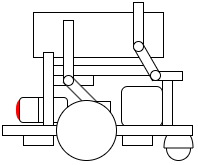
\includegraphics[scale=0.70]{images/Hardware_Mechanical/Third_Iteration_Design_side.png}
\caption{Second Iteration Side View}\label{Side View}
\endminipage
\end{figure}
\begin{figure}[htp]
\centering
\captionsetup{justification=centering}
\minipage{0.24\textwidth}
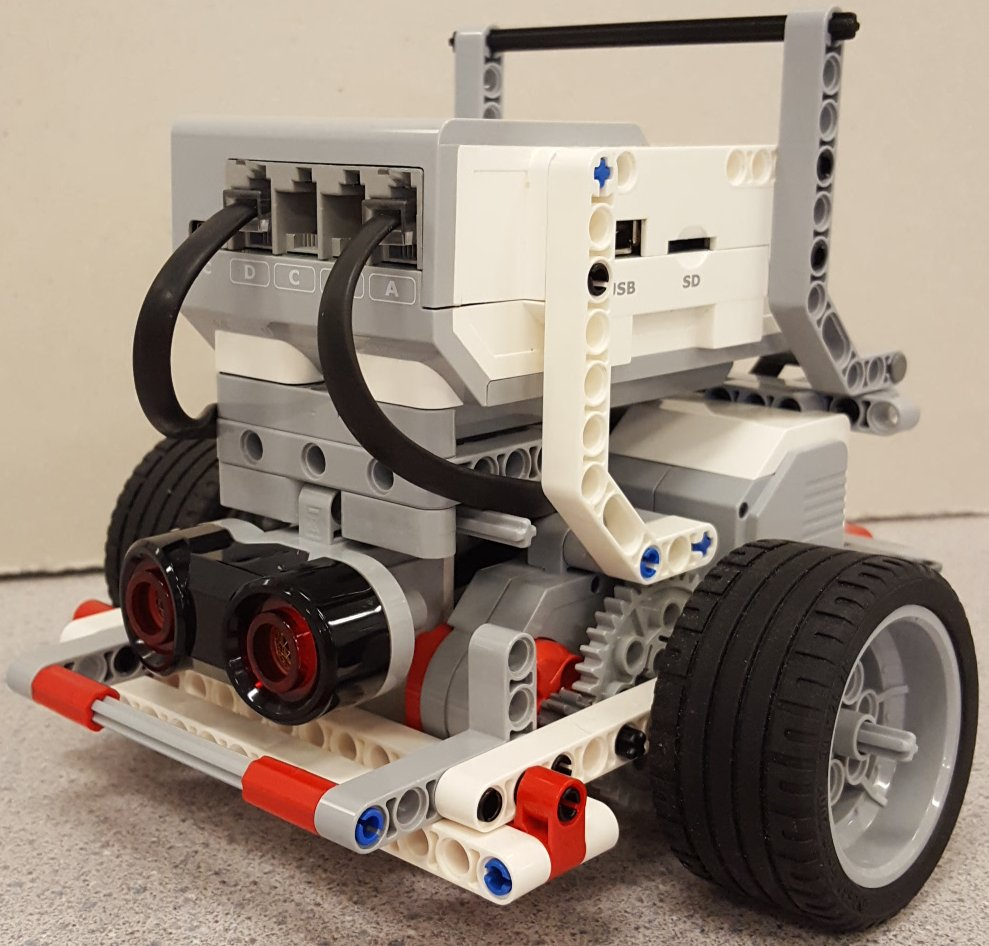
\includegraphics[scale=0.13]{images/Hardware_Mechanical/Third_Iteration_3D.jpg}
\caption{Second Iteration Drive System}\label{fig:Drive System}
\endminipage\hfill
\minipage{0.32\textwidth}
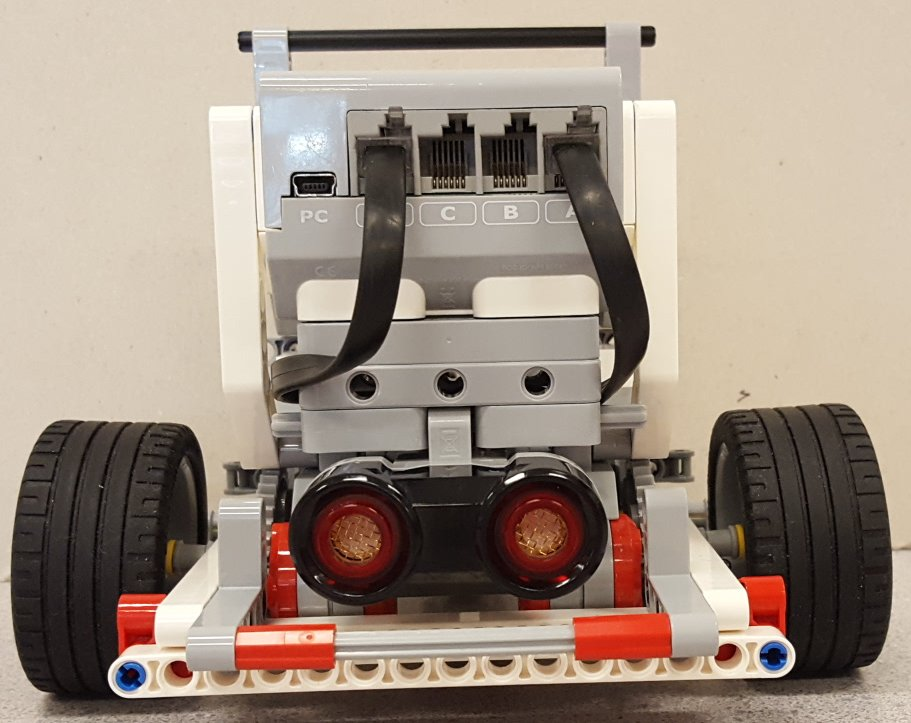
\includegraphics[scale=0.17]{images/Hardware_Mechanical/Third_Iteration_Front.jpg}
\caption{Second Iteration Front View}\label{fig:Front View}
\endminipage\hfill
\minipage{0.27\textwidth}
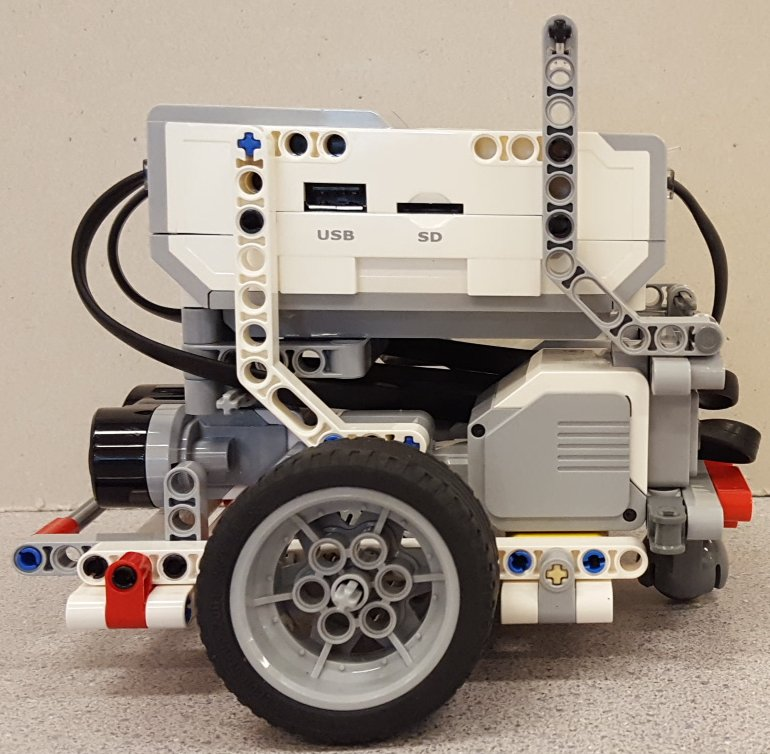
\includegraphics[scale=0.17]{images/Hardware_Mechanical/Third_Iteration_Left.jpg}
\caption{Second Iteration Side View}\label{Side View}
\endminipage
\end{figure}
\newpage
\begin{itemize}
\item \textbf{Observations \& Measurements}
	\begin{itemize}
	\item \textbf{Goal}: Able to go 3 cells without needing to readjust
 	\item \textbf{Passed}: Needed to readjust every fifth cell
 	\item \textbf{Goal}: Able to turn 90$^{\circ}$ accurately.\\
	Test - An error of even $ \pm 1^{\circ}$ will accumulate to a significant error when traversing cells. However, error in a single turn is hard to notice. Therefore, we chose to have the robot turn 90$^{\circ}$ 8 times in place in order to propagate any error significantly.
	\item \textbf{Passed}: Robot had an unnoticeable error even after eight turns
	\end{itemize}
\item \textbf{Reasons for Test Successes}\\
Our hypotheses were correct. By securing the gears, we were able to make the motor encoders much more accurate and as a result, the robot moved in a much more controlled way. Furthermore, having a more compact robot allowed the system to have a larger tolerance for movement error.
\item \textbf{Conclusion}\\
After full contemplation, we have decided that this is the best design. The need to readjust cannot be avoided because of the uncertainty in turning caused by the backlash in the gears. In order to further reduce the error, we have decided to make the algorithm for the robot as efficient as possible. An example of this is to avoid turning to check the same wall multiple times because turning is the robot's least accurate movement.
\end{itemize}
\newpage

%%%%%%%%%%%%%%%%%%%%%%%%%%%%%%%%%%%%%%%%%%%%%%%%%%%%%%%%%%%%%%
%%															%%
%% 							Section 3    					%%
%% 															%%
%%%%%%%%%%%%%%%%%%%%%%%%%%%%%%%%%%%%%%%%%%%%%%%%%%%%%%%%%%%%%%

\section{Software Design of MazeBot}
To create a program that was suitable for requirements and easy to debug, we chose to employ a lot of functions. Each function does one small task and they were tested separately. These functions were then stitched together for different phases of the robot's maze solving algorithm.\\
These phases are:\\\\
Finding solution to the maze $\to$ Solving for the shortest path $\to$ Coming back the shortest route.\\\\
Furthermore, we wanted our program to have very few constants that we would need to test. For example, in order to move forward one cell, we needed to give the following function degrees to move each of our drive motors:
\begin{verbatim}
		setMotorSyncEncoder(leftDrive, rightDrive, 0, Degrees, BACKWARD);
\end{verbatim}
The degrees needed to move one cell forward could have been calculated by constantly testing different values of degrees. However, we chose to calculate the exact degrees that is needed for the robot to move exactly one cell forward. This approach in contrast to the former has two advantages: 
\begin{enumerate}
\item It allows us to isolate any inaccurate movement problems as a purely mechanical problem.
\item We would not have an accumulation of error because of us testing incorrectly.
\end{enumerate}
Therefore, we chose to mathematically calculate the degrees that we needed to move the motors rather than testing.\\\\
A sketch of the derivation of how many degrees to move forward is shown below: %ADD SKETCH HERE% 
\begin{figure}[htp]
\centering
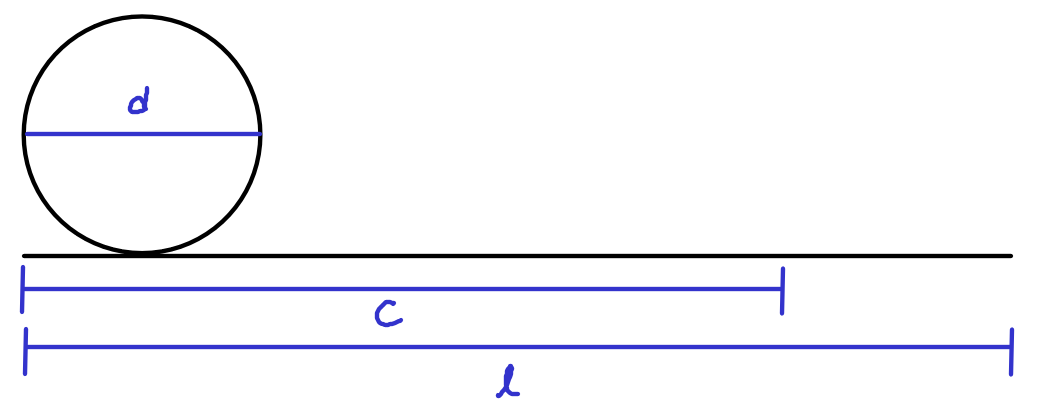
\includegraphics[scale=0.3]{images/Movement_Distance.png}
\caption{Proof of Degrees Formula}
\label{}
\end{figure}
\begin{itemize}
\item $d =$ diameter of the wheel
\item $c = d \times \pi = $ circumference of the wheel
\item $l =$ distance of one cell
\item $5$ rotations of the gear attached to the motor rotates the wheel once
\item The ratio between the distance of one cell and the circumference of the wheel is $\frac{l}{c}$
\end{itemize}
Therefore the degrees were calculated as:
\begin{verbatim}
degrees = (SIZE_OF_ONE_CELL / CIRCUMFERENCE_OF_WHEEL) * DRIVE_GEAR_RATIO * ONE_ROTATION
\end{verbatim}


%%%%%%%%%%%%%%%%%%%%%%%%%%%%%%%%%%%%%%%%%%%%%%%%%%%%%%%%%%%%%%
%%															%%
%% 					Do not remove the gap 					%%
%% 		From this, these are explanations of the code		%%
%%															%%
%%%%%%%%%%%%%%%%%%%%%%%%%%%%%%%%%%%%%%%%%%%%%%%%%%%%%%%%%%%%%%
\newpage

%% 3.1 - Position of the robot and size of the maze

\subsection{Constants and Variables Used to Define the Position of the Robot in the Maze and the Size of the Maze}
\begin{itemize}
\item Two constant that represent the initial position of the robot in the maze were declared. These will be entered when we begin our demo.
	\begin{verbatim}
		int const START_ROW = ;
		int const START_COL = ;
	\end{verbatim} 
\item Two constants that represent the target position in the maze were declared. These will be entered when we begin our demo.
	\begin{verbatim}
		int const END_ROW = ; 
		int const END_COL = ;
	\end{verbatim}
\item Two global variables that represent the current position of the robot in the maze were declared. These are initialized as the starting position. 
	\begin{verbatim}
		int currentRow = START_ROW;
		int currentCol = START_COL;
	\end{verbatim} 
\item An array that represents the orientation that the robot has as it enters each cell was defined. The size of the array is four times larger than the product of the maze width and maze height because the maximum amount of times that the robot can go into a cell is four times in the worst case scenario.
	\begin{verbatim}
		int entered[MAZE_WIDTH*MAZE_HEIGHT*4];
		int lastEnteredIdx = 0;
	\end{verbatim} 
\item A constant that represents the dimension of a single cell was defined
	\begin{verbatim}
		float const SIZE_OF_ONE_CELL = 22.5425; // in cm 	
	\end{verbatim} 
\item Four constants that represent the size of the maze were declared
	\begin{verbatim}
		int const MAZE_WIDTH = 4;
		int const MAZE_HEIGHT = 6;
		int const LAST_MAZE_HEIGHT_INDEX = MAZE_HEIGHT - 1;
		int const LAST_MAZE_WIDTH_INDEX = MAZE_WIDTH - 1;
	\end{verbatim} 
\end{itemize}
\newpage

%% 3.2

\subsection{Constants and Variables Used for Representation of Directions}
\begin{itemize}
\item The four constants that represent each of the directions were declared:
	\begin{verbatim}
		#define NORTH 0
		#define EAST 1
		#define SOUTH 2
		#define WEST 3
	\end{verbatim}
\item A structure named cell was declared and it has six parameters. For a given cell, this structure parameterized by where the walls are, whether the robot have visited the cell, and the direction that the robot entered the cell.
	\begin{verbatim}
		typedef struct{
   int NWall; 
   int SWall; 
   int EWall; 
   int WWall; 
   char Visited;
   int entryDir;
}cell;\end{verbatim}
\item A 2-D array called "Maze" with the data type cell was declared. This data type is described above.
	\begin{verbatim}
		cell Maze[MAZE_HEIGHT][MAZE_WIDTH];
	\end{verbatim}
\end{itemize}

%% 3.3

\subsection{Constants Used for Display}
\begin{itemize}
\item Two constants that represent the size of the screen width and height were defined.
	\begin{verbatim}
		#define SCREEN_HEIGHT 127
		#define SCREEN_WIDTH 177 
	\end{verbatim} 
\item Two constants that represent the single cell's size on the screen were defined.
	\begin{verbatim}
		#define CELL_HEIGHT (SCREEN_HEIGHT / MAZE_HEIGHT)
		#define CELL_WIDTH (SCREEN_WIDTH / MAZE_WIDTH)
	\end{verbatim} 
\item Two constants that represent the robot's position in each cell in the screen were defined.
	\begin{verbatim}
		#define CELL_HEIGHT_MIDDLE (CELL_HEIGHT / 2)
		#define CELL_WIDTH_MIDDLE (CELL_WIDTH /2)
	\end{verbatim}
\end{itemize}
\newpage

%% 3.4

\subsection{Constants Used for Moving Mechanism}
\begin{itemize}
\item When we calculated the degrees to move the encoder, we had three contributing errors that caused the motors to move less than they needed to. First of all, we were using integer division to find the degrees to move the motors. Therefore, the remainder is truncated and this causes the robot to move less than one cell or less than 90$^{\circ}$. Similarly, the Proportional Integral Derivative (PID) control caused the robot to move less than the desired target. Therefore, three constants were declared which are added to the encoder input values and only needed to be tested once in order to supplement the errors. 
	\begin{verbatim}
		float const UNCERTAINTY_STRAIGHT = 23;
		float const UNCERTAINTY_ROT = 28;
		float const UNCERTAINTY_READJUST = 35;
	\end{verbatim} 
\item Forward and backward speed of the motors were defined with constants for simplification of the code. 
	\begin{verbatim}
		int const FORWARD = -100;
		int const BACKWARD = -FORWARD;
	\end{verbatim} 
\item Encoder input constants were declared
	\begin{verbatim}
		float const ONE_ROTATION = 360 + UNCERTAINTY_STRAIGHT;
		float const QUARTER_ROTATION = 180 + UNCERTAINTY_ROT;
		float const DRIVE_GEAR_RATIO = 5;
		float const DIAMETER_OF_WHEEL = 5.5; // in cm
		float const CIRCUMFERENCE_OF_WHEEL = PI * DIAMETER_OF_WHEEL;
	\end{verbatim} 
\item The amount of time that the bot will drive into the wall to readjust was defined. Timing algorithm was used because the flat surface at the front of the robot adjusts the robot as it drives into the wall.
	\begin{verbatim}
		int const MILISECS_TO_DRIVE_INTO_WALL = 1100;
	\end{verbatim} 
\item A constant that represents how often the robot has to readjust was defined. A global variable that increases every time the robot goes into new cells to count for readjust was also defined.
	\begin{verbatim}
		int const CELLS_TO_READJUST_AFTER = 3;
		int timesForwardWithoutReadjust = 0;
	\end{verbatim}  
\end{itemize}
\newpage

%% 3.5

\subsection{Constants Used for Representation of Wall}
\begin{itemize}
\item A constant which represent the maximum distance possible between the robot and an object for the robot to consider it a wall in the current cell.
	\begin{verbatim}
		float const DIST_BETWEEN_BOT_AND_WALL = 7.6;
	\end{verbatim}
\item Three constants were defined that represent the robot's knowledge of whether or not there is a wall. 
	\begin{verbatim}
		#define NOT_PRESENT 0 
		#define PRESENT 1
		#define UNKNOWN 2
	\end{verbatim}
\end{itemize}

%% 3.6

\subsection{Constants Used for Beeping Mechanism}
\begin{itemize}
\item Two constants which represent the time and frequency of the beep when the robot finds the target.
	\begin{verbatim}
		int const MILI_TO_BEEP_FOR = 200;
		int const FREQUENCY = 300;
	\end{verbatim}
\end{itemize}

\newpage

%% 3.7

\subsection{Displaying Function}
\begin{itemize}
\item Function for displaying information about the robot's orientation and location on the screen. It also displays what it knows about the maze. 
	\begin{verbatim}
		void drawInfo(int direction);
	\end{verbatim}
\begin{figure}[htp]
\centering 
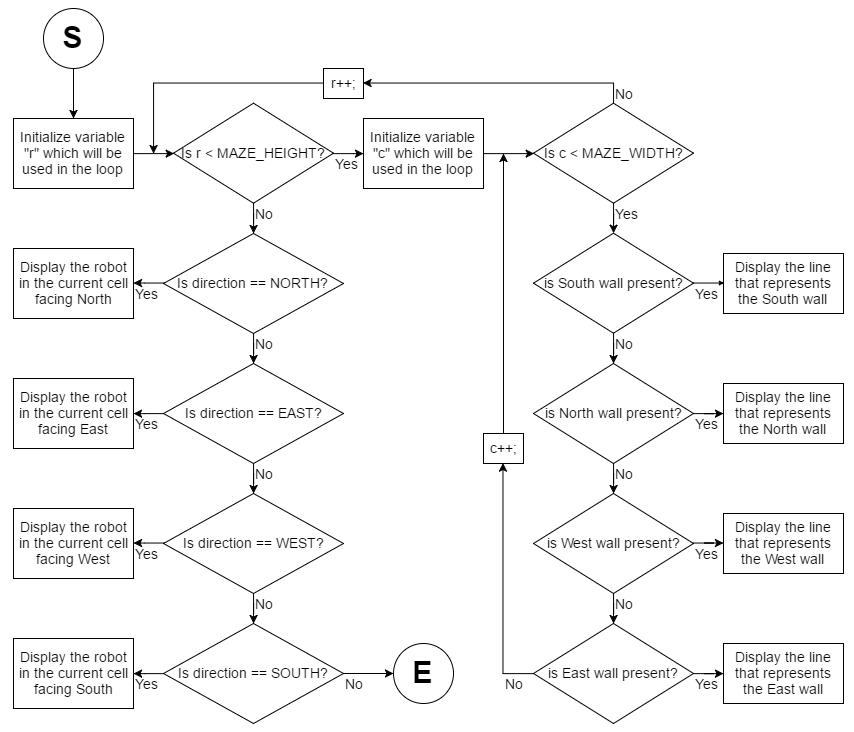
\includegraphics[scale=0.57]{images/Software_Flowchart/Drawing_Function.png}
\caption{Flow Chart for Displaying Function}
\label{}
\end{figure}
	\begin{itemize}
	\item The local variable direction is passed into the function but it does not return any variable.
	\item Global variables and constants used are:
	\begin{verbatim}
		MAZE_WIDTH     MAZE_HEIGHT
		CELL_WIDTH     CELL_HEIGHT
		CELL_WIDTH_MIDDLE     CELL_HEIGHT_MIDDLE
		Maze[][].NWall     Maze[][].SWall     Maze[][].EWall     Maze[][].WWall
	PRESENT
	currentCol     currentRow
	NORTH     SOUTH     EAST     WEST
	\end{verbatim}
	\end{itemize}
\end{itemize}
\newpage

%% 3.8

\subsection{Moving Forward Function}
\begin{itemize}
\item This function moves the the robot forward exactly one cell forward. It also stores the cell information in the maze array. Finally, it increments how many cells it has moved without readjust. 
	\begin{verbatim}
		void goFwdCell(int direction);
	\end{verbatim}
\begin{figure}[htp]
\centering
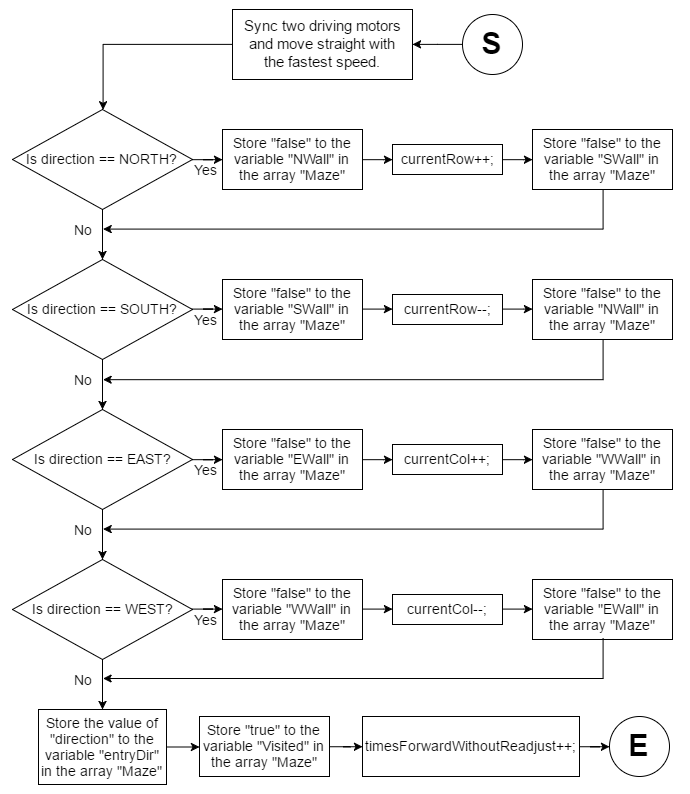
\includegraphics[scale=0.52]{images/Software_Flowchart/Moving_Forward.png}
\caption{Flow Chart for Moving Forward}
\label{}
\end{figure}	
	\begin{itemize}
	\item The local variable direction is passed into the function but it does not return any variable.
	\item Global variables and constants used are:
	\begin{verbatim}
		SIZE_OF_ONE_CELL     CIRCUMFERENCE_OF_WHEEL
		DRIVE_GEAR_RATIO     ONE_ROTATION     FORWARD
		NORTH     SOUTH     EAST     WEST
		currentCol     currentRow
		Maze[][].NWall     Maze[][].SWall     Maze[][].EWall     Maze[][].WWall
		timesForwardWithoutReadjust
	\end{verbatim}
	\end{itemize}
\end{itemize}
\newpage

%% 3.9

\subsection{Turning Functions}
\begin{itemize}
\item Function for turning right 90$^\circ$.
\begin{verbatim}
	int Turn90CW(int direction);
\end{verbatim}
\begin{figure}[htp]
\centering
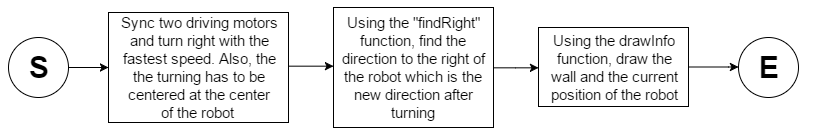
\includegraphics[scale=0.6]{images/Software_Flowchart/Turning_Right.png}
\caption{Flow Chart for Turning Right}
\label{}
\end{figure}
	\begin{itemize}
	\item The local variable direction is passed into the function. The function returns the new direction.
	\item Global constants used are:
	\begin{verbatim}
		QUARTER_ROTATION     DRIVE_GEAR_RATION
		FORWARD
	\end{verbatim}
	\item Functions called are:
	\begin{verbatim}
		int findRight(int direction);
		int drawInfo(int direction);
	\end{verbatim}
	\end{itemize}
\item Function for turning left 90$^\circ$.
\begin{verbatim}
	Turn90CW(int direction);
\end{verbatim}
\begin{figure}[htp]
\centering
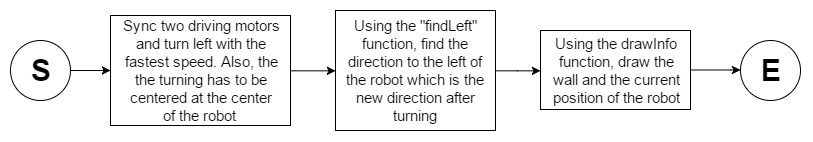
\includegraphics[scale=0.60]{images/Software_Flowchart/Turning_Left.png}
\caption{Flow Chart for Turning Left}
\label{}
\end{figure}
	\begin{itemize}
	\item The local variable direction is passed into the function. The function returns the new direction.
	\item Global constants used are:
	\begin{verbatim}
		QUARTER_ROTATION     DRIVE_GEAR_RATION
		FORWARD
	\end{verbatim}
	\item Functions called are:
	\begin{verbatim}
		int findLeft(int direction);
		int drawInfo(int direction);
	\end{verbatim}
	\end{itemize}
\end{itemize}
\newpage

%% 3.10

\subsection{Wall Detecting Function}
\begin{itemize}
\item Function that returns whether or not there is a wall in front of the robot.
	\begin{verbatim}
		int thereIsWall();
	\end{verbatim}
\begin{figure}[htp]
\centering
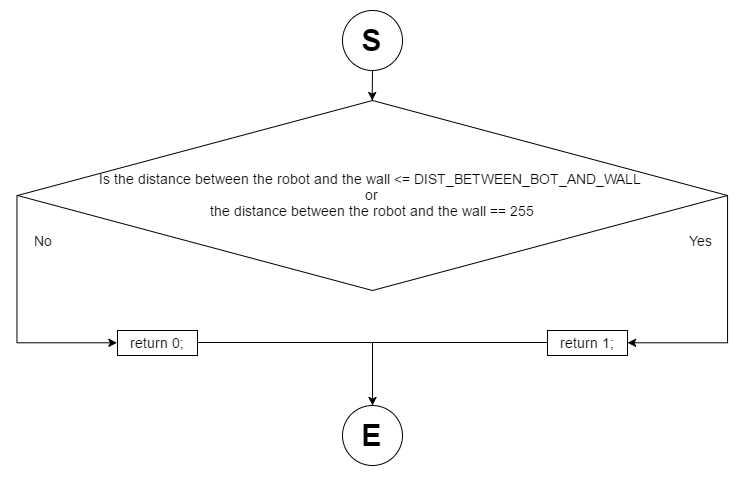
\includegraphics[scale=0.60]{images/Software_Flowchart/Detecting_Wall.png}
\caption{Flow Chart for Wall Detecting Function}
\label{}
\end{figure}
	\begin{itemize}
	\item Very simple function that returns $1$ if the sensor detects the wall.
	\item Global constant used is:
	\begin{verbatim}
		DIST_BETWEEN_BOT_AND_WALL
	\end{verbatim}
	\end{itemize}
\end{itemize}
\newpage

%% 3.11

\subsection{Function for Storing Data of the Walls}
\begin{itemize}
\item Function that writes whether there is a wall in the direction the robot is currently facing into the maze array.
	\begin{verbatim}
		void writeWall(int direction);
	\end{verbatim}
\begin{figure}[htp]
\centering
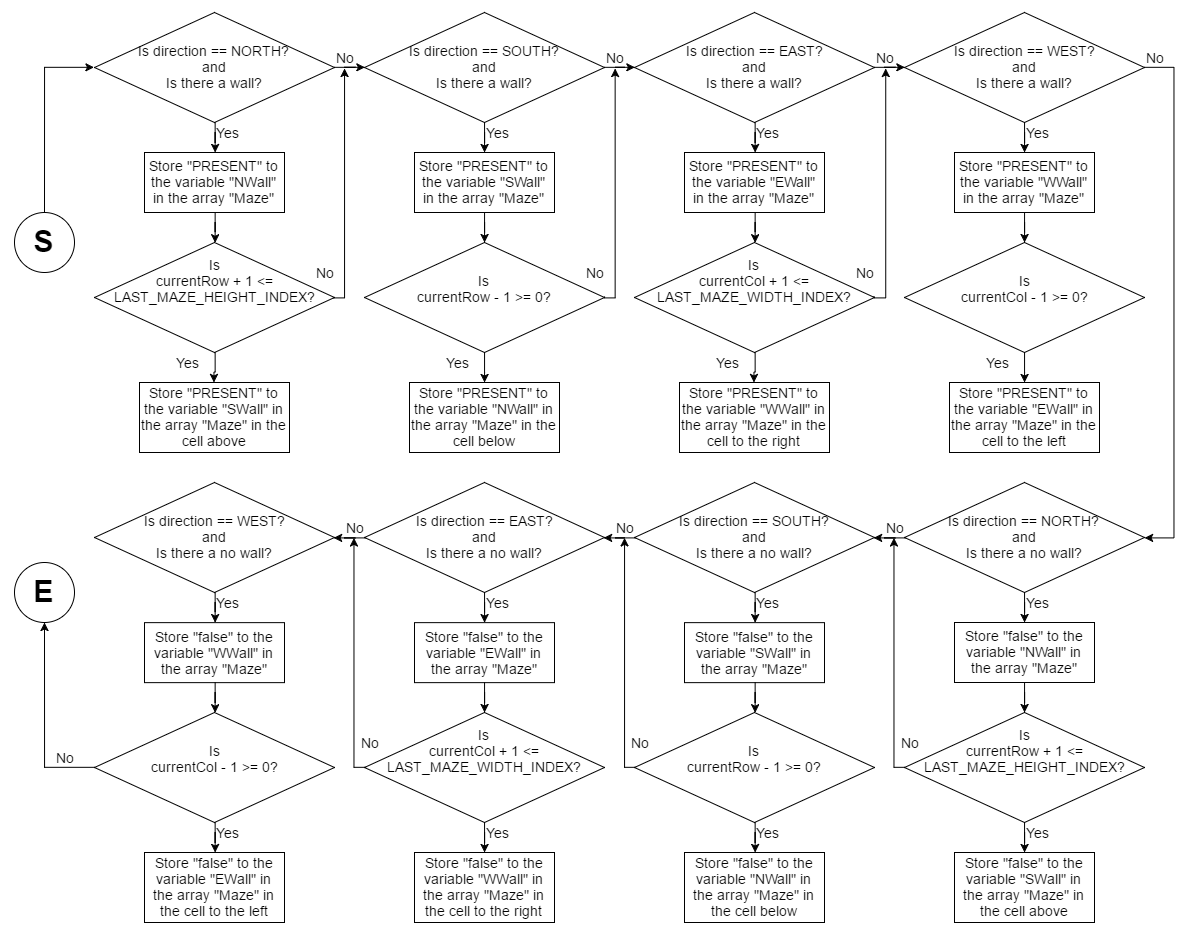
\includegraphics[scale=0.44]{images/Software_Flowchart/writeWall.png}
\caption{Flow Chart for Storing Data Function}
\label{}
\end{figure}
	\begin{itemize}
	\item The local variable direction is passed into the function but it does not return any variable.
	\item Global variables and constants used are:
	\begin{verbatim}
		NORTH     SOUTH     EAST     WEST
		currentCol     currentRow
		Maze[][].NWall     Maze[][].SWall     Maze[][].EWall     Maze[][].WWall
		PRESENT
		LAST_MAZE_HEIGHT_INDEX     LAST_MAZE_WIDTH_INDEX
	\end{verbatim}
	\item Function called is:
	\begin{verbatim}
		int thereIsWall();
	\end{verbatim}
	\end{itemize}
\end{itemize}
\newpage

%% 3.12

\subsection{Functions for setting up the direction that need to be used}
\begin{itemize}
\item Function that takes in a direction of the robot and returns the direction towards the back.
	\begin{verbatim}
		int findBackDir(int currentDirection);
	\end{verbatim}
\begin{figure}[htp]
\centering
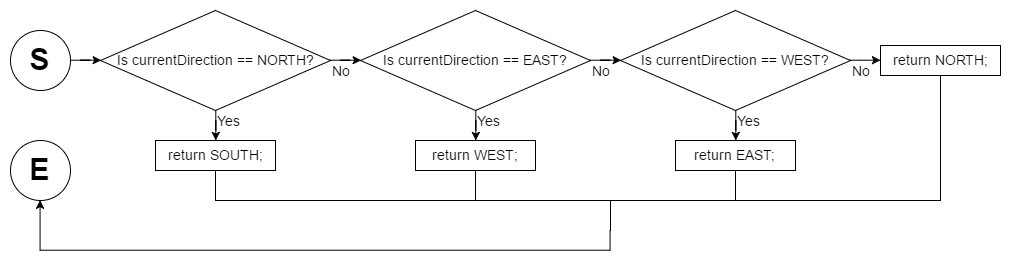
\includegraphics[scale=0.45]{images/Software_Flowchart/findBackDir.png}
\caption{Flow Chart for Finding Back Function}
\label{}
\end{figure}
\item Function that takes in a direction of the robot and returns the direction to the right of the robot.
	\begin{verbatim}
		int findRight(int currentDirection);
	\end{verbatim}
\begin{figure}[htp]
\centering
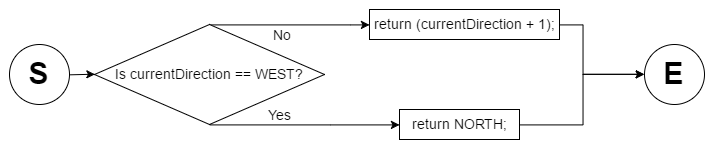
\includegraphics[scale=0.47]{images/Software_Flowchart/findRight.png}
\caption{Flow Chart for Finding Right Function}
\label{}
\end{figure}	
\item Function that takes in a direction of the robot and returns the direction to the left of the robot.
	\begin{verbatim}
		int findLeft(int currentDirection);
	\end{verbatim}
\begin{figure}[htp]
\centering
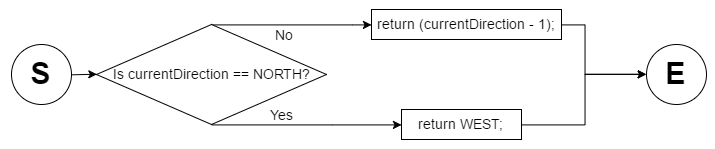
\includegraphics[scale=0.48]{images/Software_Flowchart/findLeft.png}
\caption{Flow Chart for Finding Left Function}
\label{}
\end{figure}
	\begin{itemize}
	\item Global constants used are:
	\begin{verbatim}
		NORTH     SOUTH     EAST     WEST
	\end{verbatim}
	\end{itemize}
\end{itemize}
\newpage

%% 3.13

\subsection{Functions for Finding Existence of Wall from the data}
\begin{itemize}
\item Function takes in a direction and returns whether or not there is a wall in that direction from maze array.
	\begin{verbatim}
		int isThereWallInDir(int wallDir);
	\end{verbatim}
\begin{figure}[htp]
\centering
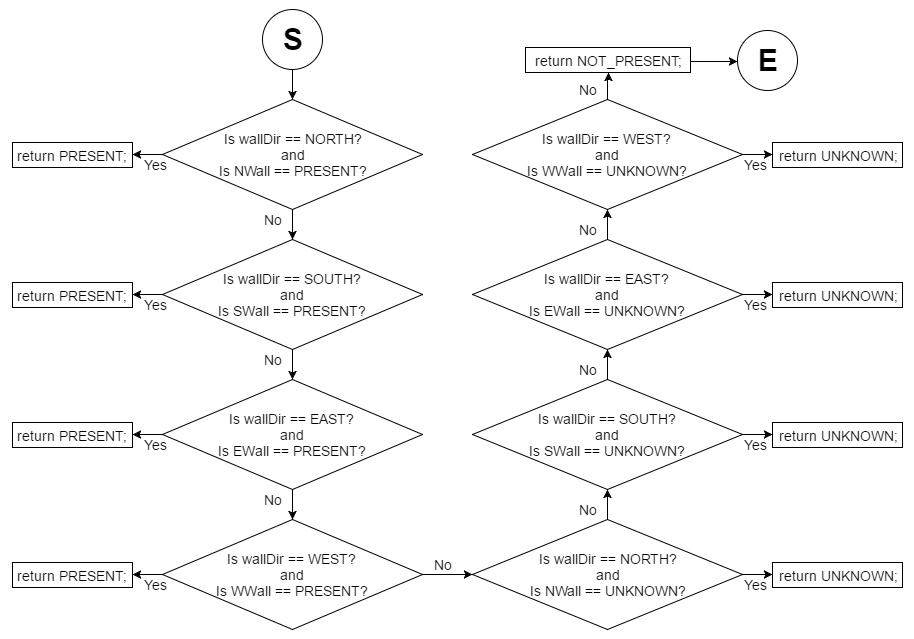
\includegraphics[scale=0.580]{images/Software_Flowchart/isThereWallInDir.png}
\caption{Flow Chart for Finding Existence of Wall from the data}
\label{}
\end{figure}
	\begin{itemize}
	\item Global variables and constants used are:
	\begin{verbatim}
		NORTH     SOUTH     EAST     WEST
		PRESENT     UNKNOWN     NOT_PRESENT
		Maze[][].NWall     Maze[][].SWall     Maze[][].EWall     Maze[][].WWall
	\end{verbatim}
	\end{itemize}
\end{itemize}
\newpage

%% 3.14

\subsection{Functions for Readjusting in Certain Directions}
\begin{itemize}
\item Function that readjusts robot's position by driving into the wall and coming back to the center of the cell. For this function particularly, we readjust using walls to the front and to the right.
	\begin{verbatim}
		void reAdjustCW(int direction);
	\end{verbatim}
\begin{figure}[htp]
\centering
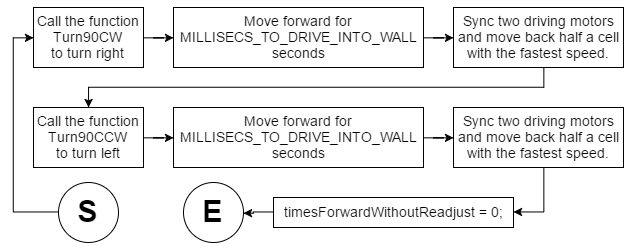
\includegraphics[scale=0.52]{images/Software_Flowchart/reAdjustCW.png}
\caption{Flow Chart for Readjusting using Front wall and Right wall}
\label{}
\end{figure}
\item Function that readjusts robot's position by driving into the wall and coming back to the center of the cell. For this function particularly, we readjust using walls to the back and to the left.
	\begin{verbatim}
		void reAdjustCCW(int direction);
	\end{verbatim}
\begin{figure}[htp]
\centering
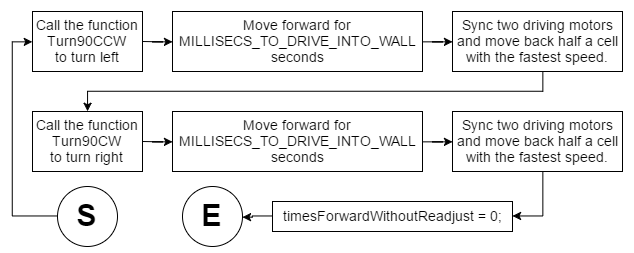
\includegraphics[scale=0.52]{images/Software_Flowchart/reAdjustCCW.png}
\caption{Flow Chart for Readjusting using Back wall and Left wall}
\label{}
\end{figure}
	\begin{itemize}
	\item The local variable direction is passed into the function but it does not return any variable.
	\item Global variables and constants used are:
	\begin{verbatim}
		SIZE_OF_ONE_CELL     CIRCUMFERENCE_OF_WHEEL
		DRIVE_GEAR_RATIO     ONE_ROTATION     UNCERTAINTY_READJUST
		FORWARD     BACKWARD     MILLISECS_TO_DRIVE_INTO_WALL
		NORTH     SOUTH     EAST     WEST
		Maze[][].NWall     Maze[][].SWall     Maze[][].EWall     Maze[][].WWall
		timesForwardWithoutReadjust
	\end{verbatim}
	\item Functions called are:
	\begin{verbatim}
		int Turn90CW(int direction);
		int Turn90CCW(int direction);
	\end{verbatim}
	\end{itemize}
\item Function that decides which direction to readjust using the data collected in the array. Once the function decides the direction to readjust in, it calls that function.
	\begin{verbatim}
		void reAdjustWayBack(int direction);
	\end{verbatim}
\begin{figure}[htp]
\centering
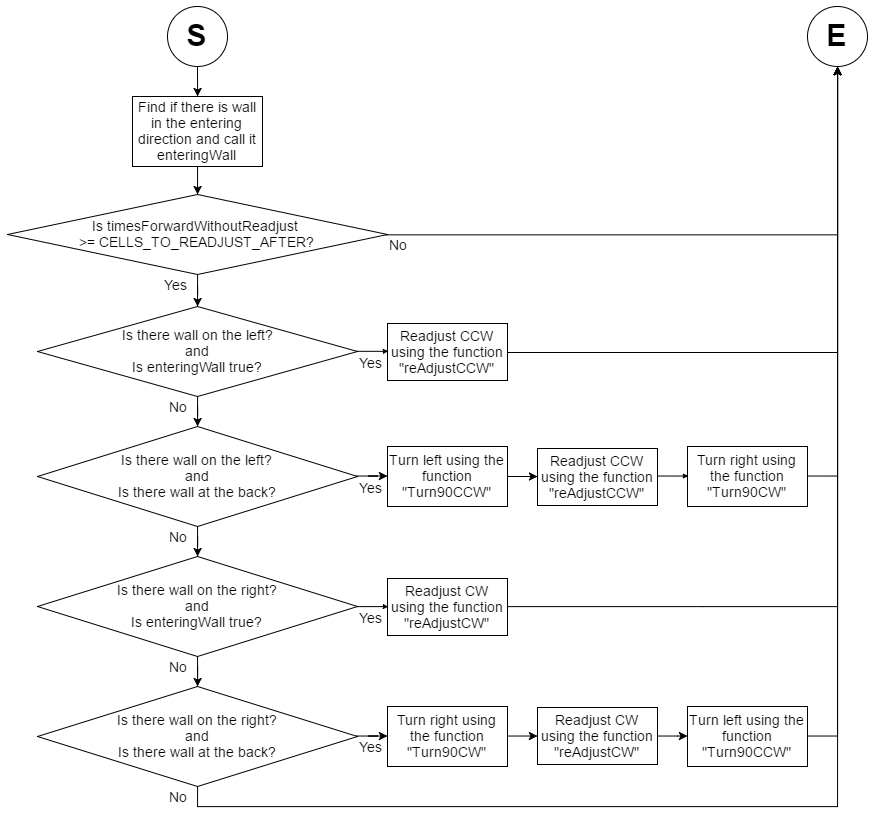
\includegraphics[scale=0.47]{images/Software_Flowchart/reAdjustWayBack.png}
\caption{Flow Chart for Readjusting using walls detected}
\label{}
\end{figure}
	\begin{itemize}
	\item The local variable direction is passed into the function but it does not return any variable.
	\item Global variable and constants used are:
	\begin{verbatim}
		timesForwardWithoutReadjust
		CELLS_TO_READJUST_AFTER
		PRESENT
	\end{verbatim}
	\item Functions called are:
	\begin{verbatim}
		thereIsWall();
		reAdjustCW(int direction);
		reAdjustCCW(int direction);
		findLeft(int currentDirection);
		findRight(int currentDirection);
		findBackDir(int currentDirection);
		isThereWallInDir(int wallDir);
	\end{verbatim}
	\end{itemize}
\end{itemize}
\newpage

%% 3.15

\subsection{Function for Movement All Together}
\begin{itemize}
\item Function that implements the right following algorithm using the functions described above. Furthermore, it ensures that the robot readjusts whenever it can.
	\begin{verbatim}
		int MovementWithSensor(int direction);
	\end{verbatim}
\begin{figure}[htp]
\centering
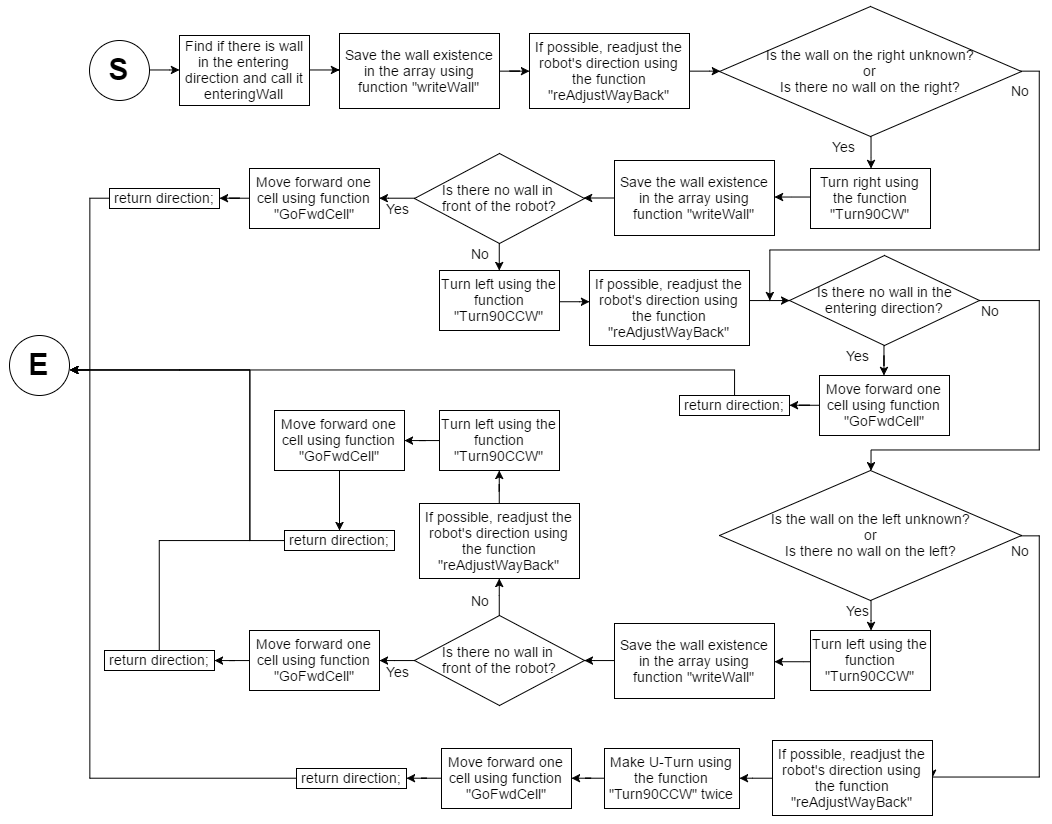
\includegraphics[scale=0.47]{images/Software_Flowchart/MovementWithSensor.png}
\caption{Flow Chart for Movement Function}
\label{}
\end{figure}
	\begin{itemize}
	\item The local variable direction is passed into the function and it returns a new variable direction.
	\item Global constants used are:
	\begin{verbatim}
		NOT_PRESENT     UNKNOWN
	\end{verbatim}
	\item Functions called are: 
	\begin{verbatim}
		writewall(int direction);
		reAdjustWayBack(int direction);
		isThereWallInDir(int wallDir);
		findRight(int currentDirection);
		thereIsWall();
		goFwdCell(int direction);
		Turn90CCW(int direction);
		Turn90CW(int direction);
	\end{verbatim}
	\end{itemize}
\end{itemize}
\newpage

%% 3.16

\subsection{Functions for Returning Algorithm}
\begin{itemize}
\item Function that deletes the duplicates from the array which saved up how the robot entered each cell. For example, if the robot moved two opposite directions in order, it is not necessary to follow those directions. Therefore, we delete the duplicates from the array.
 	\begin{verbatim}
		void deleteDuplicates();
	\end{verbatim}
\begin{figure}[htp]
\centering
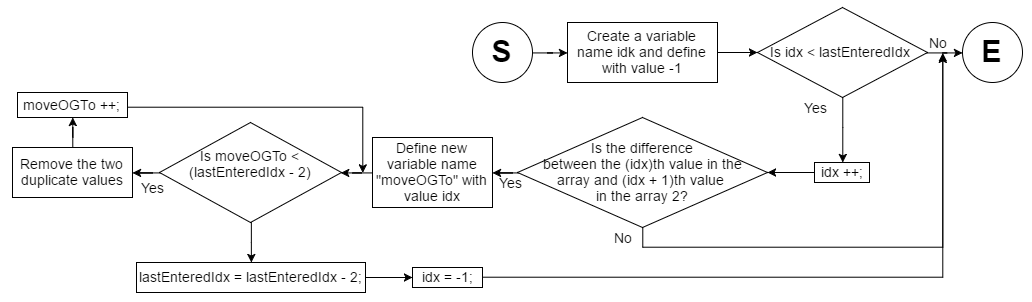
\includegraphics[scale=0.50]{images/Software_Flowchart/deleteDuplicate.png}
\caption{Flow Chart for Deleting Duplicate Function}
\label{}
\end{figure}
	\begin{itemize}
	\item Global variables used are:
 		\begin{verbatim}
			entered[]     lastEnteredIdx
		\end{verbatim}
	\end{itemize}
\item Function that reverses the direction from the array which saved up how the robot entered each cell. For example, if the robot went into the cell with direction East, then we change it to West. Therefore, we change all the directions to its opposite.
 	\begin{verbatim}
		void reverseDirection();
	\end{verbatim}
\begin{figure}[htp]
\centering
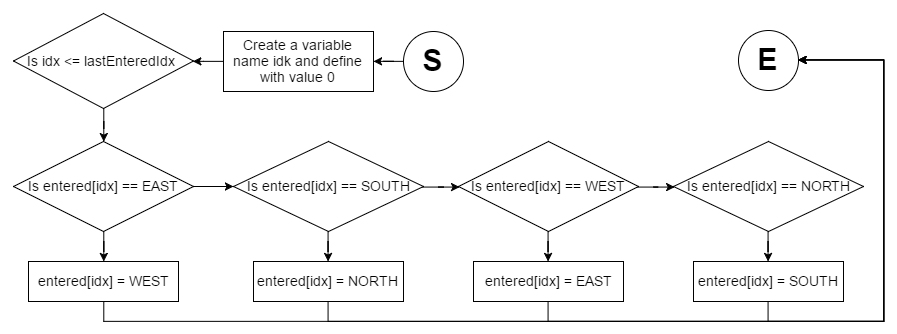
\includegraphics[scale=0.50]{images/Software_Flowchart/reverseDirection.png}
\caption{Flow Chart for Reversing Order of Values in the Array}
\label{}
\end{figure}
	\begin{itemize}
	\item Global variables and constants used are:
 		\begin{verbatim}
			entered[]     lastEnteredIdx
			NORTH     SOUTH     EAST     WEST
		\end{verbatim}
	\end{itemize}
\item Function that takes in the variable direction and goes back to the initial position in the cell with the new array created by the two functions above.
 	\begin{verbatim}
		void goingBackFastestRoute(int direction);
	\end{verbatim}
\begin{figure}[htp]
\centering
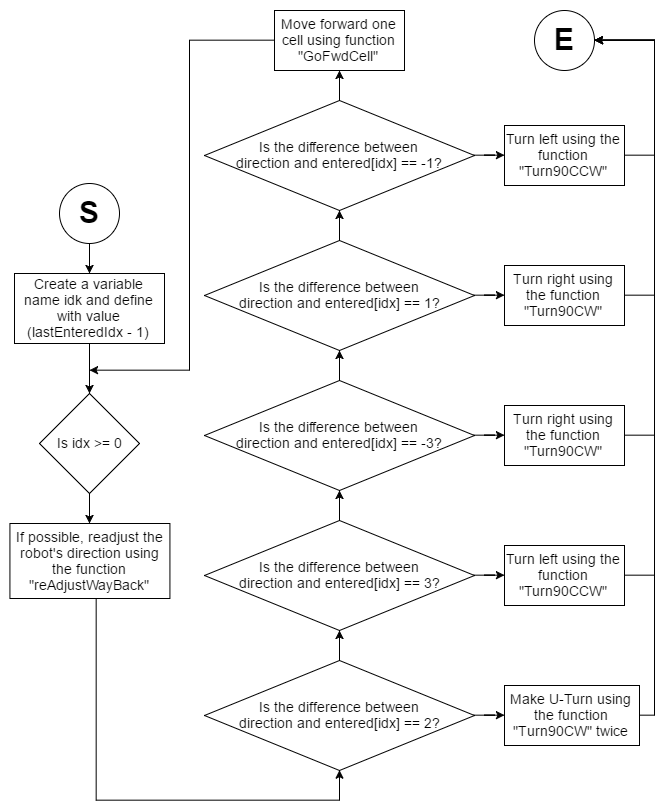
\includegraphics[scale=0.53]{images/Software_Flowchart/goingBackFastestRoute.png}
\caption{Flow Chart for Function to Go Back to Initial Position}
\label{}
\end{figure}
	\begin{itemize}
	\item Global variables and constants used are:
	\begin{verbatim}
		entered[]     lastEnteredIdx
		NORTH     SOUTH     EAST     WEST
	\end{verbatim}
	\item Functions called are:
	\begin{verbatim}
		reAdjustWayBack(int direction);	
		Turn90CW(int direction);
		Turn90CCW(int direction);
		goFwdCell(int direction);
	\end{verbatim}
	\end{itemize}
\end{itemize}
\newpage

%% 3.17

\subsection{Main Function}
\begin{itemize}
\item More than ten functions were declared for simplicity of the main function. This function calls all the smaller functions.
	\begin{verbatim}
		task main()
	\end{verbatim}
	\begin{itemize}
	\item A variable that represents current direction of the robot was declared. This is initialized as north as this is the orientation of the robot when it first enters the maze.
	\begin{verbatim}
		int direction = NORTH;
	\end{verbatim}
	\item Global variables and constants used are:
	\begin{verbatim}
		MAZE_WIDTH     MAZE_HEIGHT
		entered[]     lastEnteredIdx
		FREQUENCY     MILI_TO_BEEP_FOR
		Maze[][].NWall     Maze[][].SWall     Maze[][].EWall     Maze[][].WWall
		Maze[][].entryDir     Maze[][].Visited
		PRESENT     UNKNOWN
		LAST_MAZE_HEIGHT_INDEX     LAST_MAZE_WIDTH_INDEX 
		currentCol     currentRow    				
	\end{verbatim}
	\item Functions called are:
	\begin{verbatim}
		MovmentWithSensor(int direction);
		deleteDuplicates();
		reverseDirection();
		goingBackFastestRoute(int direction);
		drawInfo(int direction);
	\end{verbatim}
	\end{itemize}
\item Flow chart is on the next page.
\end{itemize}
\begin{figure}[htp]
\centering
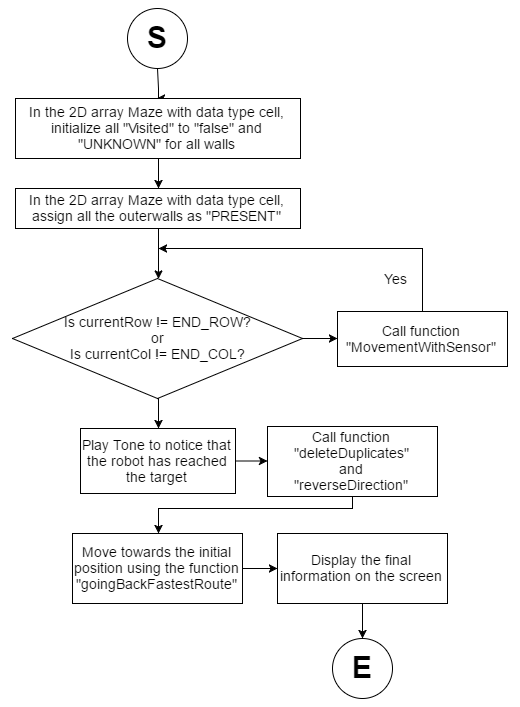
\includegraphics[scale=0.7]{images/Software_Flowchart/task_main.png}
\caption{Flow Chart of the Main Function}
\label{}
\end{figure}
\newpage


%%%%%%%%%%%%%%%%%%%%%%%%%%%%%%%%%%%%%%%%%%%%%%%%%%%%%%%%%%%%%%
%%															%%
%% 							Section 4    					%%
%% 															%%
%%%%%%%%%%%%%%%%%%%%%%%%%%%%%%%%%%%%%%%%%%%%%%%%%%%%%%%%%%%%%%


\section{Appendix}
\subsection{Full Source Code}

\begin{linenumbers}
\begin{verbatim}
    #pragma config(Sensor, S1, distance, sensorEV3_Ultrasonic)
    #pragma config(Motor, motorA, leftDrive, tmotorEV3_Large, PIDControl, driveLeft, encoder)
    #pragma config(Motor, motorD, rightDrive, tmotorEV3_Large, PIDControl, driveRight, encoder)
    //*!!Code automatically generated by 'ROBOTC' configuration wizard               !!*//

    // Constants for robot's knowledge
    #define NOT_PRESENT 0
    #define PRESENT 1
    #define UNKNOWN 2

    // Maximum distance between robot and the wall
    float const DIST_BETWEEN_BOT_AND_WALL = 7.6;

    // Define directions using numbers
    #define NORTH 0
    #define EAST 1
    #define SOUTH 2
    #define WEST 3

    typedef struct{
        int NWall;
        int SWall;
        int EWall;
        int WWall;
        int Visited;
        int entryDir;
    }cell;

    // Starting and End positions defined with Row and Column numbers
    // These positions were used for the Demo
    int const START_ROW = 2;
    int const START_COL = 0;
    int const END_ROW = 3;
    int const END_COL = 4;
    // (3,0) to (3,4) - longest route was the longest path for the practice

    // Current position defined
    int currentRow = START_ROW;
    int currentCol = START_COL;

    // Constants for beeping mechanism
    int const MILI_TO_BEEP_FOR = 200;
    int const FREQUENCY = 300;

    // Uncertainty due to property of integer division of computer
    float const UNCERTAINTY_STRAIGHT = 19;
    float const UNCERTAINTY_ROT = 27;
    float const UNCERTAINTY_READJUST = 35;

    // Movement Variabels defined
    float const ONE_ROTATION = 360 + UNCERTAINTY_STRAIGHT;
    float const QUARTER_ROTATION = 180 + UNCERTAINTY_ROT;
    float const SIZE_OF_ONE_CELL = 22.5425; //cm
    float const DRIVE_GEAR_RATIO = 5;
    float const DIAMETER_OF_WHEEL = 5.5; // cm
    float const CIRCUMFERENCE_OF_WHEEL = PI * DIAMETER_OF_WHEEL;

    // Speed Variable
    int const FORWARD = -100;
    int const BACKWARD = -FORWARD;

    // MAZE VARIABLES
    int const MAZE_WIDTH = 6;
    int const MAZE_HEIGHT = 4;
    int const LAST_MAZE_HEIGHT_INDEX = MAZE_HEIGHT - 1;
    int const LAST_MAZE_WIDTH_INDEX = MAZE_WIDTH - 1;
    cell Maze[MAZE_HEIGHT][MAZE_WIDTH];

    // Array to save up how the robot entered each cells
    int entered[MAZE_WIDTH*MAZE_HEIGHT*4];
    int lastEnteredIdx = 0;

    // Constants for displaying mechanism
    #define SCREEN_HEIGHT 127
    #define	SCREEN_WIDTH 177
    #define CELL_HEIGHT	(SCREEN_HEIGHT / MAZE_HEIGHT)
    #define CELL_WIDTH (SCREEN_HEIGHT / MAZE_WIDTH)
    #define CELL_HEIGHT_MIDDLE (CELL_HEIGHT / 2)
    #define CELL_WIDTH_MIDDLE (CELL_WIDTH / 2)

    // Constants for readjusting mechanism
    int const MILLISECS_TO_DRIVE_INTO_WALL = 1100;
    int const CELLS_TO_READJUST_AFTER = 3;
    int timesForwardWithoutReadjust = 0;

    // Call functions
    void goFwdCell(int direction);
    int Turn90CW(int direction);
    int Turn90CCW(int direction);
    int MovementWithSensor(int direction);
    void reverseDirection();
    void deleteDuplicates();
    int goingBackFastestRoute(int direction);
    void drawInfo(int direction);
    void reAdjustCCW(int direction);
    void reAdjustCW(int direction);
    int findLeft(int currentDirection);
    int findRight(int currentDirection);
    int findBackDir (int currentDirection);
    int isThereWallInDir(int wallDir);
    void reAdjustWayBack(int direction);


    void drawInfo(int direction){
        eraseDisplay();

        for(int r = 0; r < MAZE_HEIGHT; r++){
            for(int c = 0; c < MAZE_WIDTH; c++){

                if(Maze[r][c].SWall == PRESENT){
                    drawLine(c*CELL_WIDTH,r*CELL_HEIGHT,c*CELL_WIDTH + CELL_WIDTH,r*CELL_HEIGHT);
                }
                if(Maze[r][c].NWall == PRESENT){
                    drawLine(c*CELL_WIDTH,r*CELL_HEIGHT + CELL_HEIGHT,
                             c*CELL_WIDTH + CELL_WIDTH,r*CELL_HEIGHT + CELL_HEIGHT);
                }
                if(Maze[r][c].WWall == PRESENT){
                    drawLine(c*CELL_WIDTH,r*CELL_HEIGHT,c*CELL_WIDTH,
                             r*CELL_HEIGHT + CELL_HEIGHT);
                }
                if(Maze[r][c].EWall == PRESENT){
                    drawLine(c*CELL_WIDTH + CELL_WIDTH,r*CELL_HEIGHT,
                             c*CELL_WIDTH + CELL_WIDTH, r*CELL_HEIGHT + CELL_HEIGHT);
                }
            }
        }

        if(direction == NORTH){
            displayBigStringAt(currentCol*CELL_WIDTH + CELL_WIDTH_MIDDLE, 
                               currentRow*CELL_HEIGHT + CELL_HEIGHT_MIDDLE, "^");
        }
        else if(direction == EAST){
            displayBigStringAt(currentCol*CELL_WIDTH + CELL_WIDTH_MIDDLE,
                               currentRow*CELL_HEIGHT + CELL_HEIGHT_MIDDLE, ">");
        }
        else if(direction == WEST){
            displayBigStringAt(currentCol*CELL_WIDTH + CELL_WIDTH_MIDDLE,
                               currentRow*CELL_HEIGHT + CELL_HEIGHT_MIDDLE, "<");
        }
        else if(direction == SOUTH){
            displayBigStringAt(currentCol*CELL_WIDTH + CELL_WIDTH_MIDDLE,
                               currentRow*CELL_HEIGHT + CELL_HEIGHT_MIDDLE, "v");
        }
    }





    task main(){

        for (int c = 0; c < MAZE_WIDTH; c++){
            for (int r = 0; r < MAZE_HEIGHT; r++){
                Maze[r][c].Visited = false;
                Maze[r][c].NWall = UNKNOWN;
                Maze[r][c].SWall = UNKNOWN;
                Maze[r][c].EWall = UNKNOWN;
                Maze[r][c].WWall = UNKNOWN;
            }
        }

        // Assigning walls [row][col]
        for (int c = 0; c < MAZE_WIDTH; c++){
            Maze[0][c].SWall = PRESENT;
            Maze[LAST_MAZE_HEIGHT_INDEX][c].NWall = PRESENT;
        }

        for (int r = 0; r < MAZE_HEIGHT; r++){
            Maze[r][0].WWall = PRESENT;
            Maze[r][LAST_MAZE_WIDTH_INDEX].EWall = PRESENT;
        }

        int direction = NORTH;

        Maze[currentRow][currentCol].entryDir = direction;
        Maze[currentRow][currentCol].Visited = true;

        while(currentRow != END_ROW || currentCol != END_COL){
            direction = MovementWithSensor(direction);
            entered[lastEnteredIdx] = direction;
            lastEnteredIdx++;
        }

        playTone(FREQUENCY, MILI_TO_BEEP_FOR);

        deleteDuplicates();

        sleep(MILI_TO_BEEP_FOR * 10);

        reverseDirection();
        
        direction = goingBackFastestRoute(direction);

        drawInfo(direction);

        sleep(390000);
    }



    void deleteDuplicates(){
        int idx = -1;

        while(idx < lastEnteredIdx){
            idx++;

            if(abs(entered[idx] - entered[idx + 1]) == 2){
                for(int moveOGTo = idx; moveOGTo <= lastEnteredIdx - 2; moveOGTo++){
                    entered[moveOGTo] = entered[moveOGTo + 2];
                }
                lastEnteredIdx = lastEnteredIdx - 2;
                idx = -1;
            }
        }
    }


    void reverseDirection(){
        for(int idx = 0; idx <= lastEnteredIdx; idx++){
            if(entered[idx]==EAST){
                entered[idx] = WEST;
            }
            else if(entered[idx]==SOUTH){
                entered[idx] = NORTH;
            }
            else if(entered[idx]==WEST){
                entered[idx] = EAST;
            }
            else if(entered[idx]==NORTH){
                entered[idx] = SOUTH;
            }
        }
    }


    int goingBackFastestRoute(int direction){

        for(int idx = lastEnteredIdx - 1; idx >= 0; idx--){
            reAdjustWayBack(direction);
            int turnNum = entered[idx] - direction;

            if(abs(turnNum) == 2){
                direction = Turn90CW(direction);
                direction = Turn90CW(direction);
            }
            else if(turnNum == 3){
                direction = Turn90CCW(direction);
            }
            else if(turnNum == -3){
                direction = Turn90CW(direction);
            }
            else if(turnNum == 1){
                direction = Turn90CW(direction);
            }
            else if(turnNum == -1){
                direction = Turn90CCW(direction);
            }
            goFwdCell(direction);
        }
        return direction;
    }


    void goFwdCell(int direction){
        setMotorSyncEncoder(leftDrive, rightDrive, 0, 
                            (SIZE_OF_ONE_CELL / CIRCUMFERENCE_OF_WHEEL)*DRIVE_GEAR_RATIO 
                            * ONE_ROTATION, FORWARD);

        repeatUntil(!getMotorRunning(leftDrive) && !getMotorRunning(rightDrive)){

        }
        if (direction == NORTH){
            Maze[currentRow][currentCol].NWall = false;
            currentRow++;
            Maze[currentRow][currentCol].SWall = false;
        }
        else if (direction == SOUTH){
            Maze[currentRow][currentCol].SWall = false;
            currentRow--;
            Maze[currentRow][currentCol].NWall = false;
        }
        else if (direction == EAST){
            Maze[currentRow][currentCol].EWall = false;
            currentCol++;
            Maze[currentRow][currentCol].WWall = false;
        }
        else if (direction == WEST){
            Maze[currentRow][currentCol].WWall = false;
            currentCol--;
            Maze[currentRow][currentCol].EWall = false;
        }

        Maze[currentRow][currentCol].entryDir = direction;
        Maze[currentRow][currentCol].Visited = true;

        timesForwardWithoutReadjust++;
    }





    int Turn90CCW(int direction){
        setMotorSyncEncoder(leftDrive, rightDrive, -100, QUARTER_ROTATION * DRIVE_GEAR_RATIO, 
                            FORWARD);

        repeatUntil(!getMotorRunning(leftDrive) && !getMotorRunning(rightDrive)){

        }
        direction = findLeft(direction);
        drawInfo(direction);
        return direction;
    }


    int Turn90CW(int direction){
        setMotorSyncEncoder(leftDrive, rightDrive, 100, QUARTER_ROTATION * DRIVE_GEAR_RATIO,
                            FORWARD);

        repeatUntil(!getMotorRunning(leftDrive) && !getMotorRunning(rightDrive)){

        }
        direction = findRight(direction);
        drawInfo(direction);
        return direction;
    }


    int thereIsWall(){
        if(getUSDistance(distance)<=DIST_BETWEEN_BOT_AND_WALL || getUSDistance(distance)==255){
            return 1;
        }
        return 0;
    }


    void writeWall(int direction){
        if(direction == NORTH && thereIsWall()){
            Maze[currentRow][currentCol].NWall = PRESENT;
            if(currentRow + 1 <= LAST_MAZE_HEIGHT_INDEX){
                Maze[currentRow + 1][currentCol].SWall = PRESENT;
            }
        }
        else if(direction == SOUTH && thereIsWall()){
            Maze[currentRow][currentCol].SWall = PRESENT;
            if(currentRow - 1 >= 0){
                Maze[currentRow - 1][currentCol].NWall = PRESENT;
            }
        }
        else if(direction == EAST && thereIsWall()){
            Maze[currentRow][currentCol].EWall = PRESENT;
            if(currentCol + 1 <= LAST_MAZE_WIDTH_INDEX){
                Maze[currentRow][currentCol + 1].WWall = PRESENT;
            }
        }
        else if(direction == WEST && thereIsWall()){
            Maze[currentRow][currentCol].WWall = PRESENT;
            if(currentCol - 1 >= 0){
                Maze[currentRow][currentCol - 1].EWall = PRESENT;
            }
        }
        else if(direction == NORTH && !thereIsWall()){
            Maze[currentRow][currentCol].NWall = false;
            if(currentRow + 1 <= LAST_MAZE_HEIGHT_INDEX){
                Maze[currentRow + 1][currentCol].SWall = false;
            }
        }
        else if(direction == SOUTH && !thereIsWall()){
            Maze[currentRow][currentCol].SWall = false;
            if(currentRow - 1 >= 0){
                Maze[currentRow - 1][currentCol].NWall = false;
            }
        }
        else if(direction == EAST && !thereIsWall()){
            Maze[currentRow][currentCol].EWall = false;
            if(currentCol + 1 <= LAST_MAZE_WIDTH_INDEX){
                Maze[currentRow][currentCol + 1].WWall = false;
            }
        }
        else if(direction == WEST && !thereIsWall()){
            Maze[currentRow][currentCol].WWall = false;
            if(currentCol - 1 >= 0){
                Maze[currentRow][currentCol - 1].EWall = false;
            }
        }	
    }


    // Checking order, North(0), East(1), West(3) then South(2)
    // right, north, left, back
    int MovementWithSensor(int direction){

        int enteringDirectionWall = thereIsWall();
        writeWall(direction);
        reAdjustWayBack(direction);
        
        // turn to check if wall is right
        if(isThereWallInDir(findRight(direction)) == UNKNOWN 
           || isThereWallInDir(findRight(direction)) == NOT_PRESENT){
            direction = Turn90CW(direction);
            writeWall(direction);
            
            // go right if no wall right
            if(!thereIsWall()){
                goFwdCell(direction);
                return direction;
            }
            else{
                direction = Turn90CCW(direction);
                reAdjustWayBack(direction);
            }
        }		
        if(!enteringDirectionWall){
                goFwdCell(direction);
                return direction;
        }
        
        // At this point, we know there r walls on the R and N
        // We are facing N 
        // if we know there is wall left, go thru back
        if(isThereWallInDir(findLeft(direction)) == UNKNOWN 
           || isThereWallInDir(findLeft(direction)) == NOT_PRESENT){
           
            direction = Turn90CCW(direction);
            writeWall(direction);
                            
            if(!thereIsWall()){
                goFwdCell(direction);
                return direction;
            }
            else{
                reAdjustWayBack(direction);
                direction = Turn90CCW(direction);
                goFwdCell(direction);
                return direction;
            }	
        }
        else{
            reAdjustWayBack(direction);
            direction = Turn90CCW(direction);
            direction = Turn90CCW(direction);
            goFwdCell(direction);
            return direction;
        }
        sleep(1000000);
    }









    void reAdjustCCW(int direction){

        direction = Turn90CCW(direction);
        motor[rightDrive] = FORWARD;
        motor[leftDrive] = FORWARD;
        sleep(MILLISECS_TO_DRIVE_INTO_WALL);

        setMotorSyncEncoder(leftDrive, rightDrive, 0, ((SIZE_OF_ONE_CELL / CIRCUMFERENCE_OF_WHEEL)
                            *DRIVE_GEAR_RATIO * ONE_ROTATION)/7 + UNCERTAINTY_READJUST,
                             BACKWARD);

        repeatUntil(!getMotorRunning(leftDrive) && !getMotorRunning(rightDrive)){

        }
        Turn90CW(direction);
        motor[rightDrive] = FORWARD;
        motor[leftDrive] = FORWARD;
        sleep(MILLISECS_TO_DRIVE_INTO_WALL);

        setMotorSyncEncoder(leftDrive, rightDrive, 0, 
                            ((SIZE_OF_ONE_CELL / CIRCUMFERENCE_OF_WHEEL)*DRIVE_GEAR_RATIO 
                            * ONE_ROTATION)/7 + UNCERTAINTY_READJUST, BACKWARD);

        repeatUntil(!getMotorRunning(leftDrive) && !getMotorRunning(rightDrive)){

        }
        timesForwardWithoutReadjust = 0;
    }


    void reAdjustCW(int direction){

        direction = Turn90CW(direction);
        motor[rightDrive] = FORWARD;
        motor[leftDrive] = FORWARD;
        sleep(MILLISECS_TO_DRIVE_INTO_WALL);

        setMotorSyncEncoder(leftDrive, rightDrive, 0,
                            ((SIZE_OF_ONE_CELL / CIRCUMFERENCE_OF_WHEEL)*DRIVE_GEAR_RATIO 
                            * ONE_ROTATION)/7 + UNCERTAINTY_READJUST, BACKWARD);

        repeatUntil(!getMotorRunning(leftDrive) && !getMotorRunning(rightDrive)){

        }
        Turn90CCW(direction);
        motor[rightDrive] = FORWARD;
        motor[leftDrive] = FORWARD;
        sleep(MILLISECS_TO_DRIVE_INTO_WALL);

        setMotorSyncEncoder(leftDrive, rightDrive, 0,
                            ((SIZE_OF_ONE_CELL / CIRCUMFERENCE_OF_WHEEL)*DRIVE_GEAR_RATIO 
                            * ONE_ROTATION)/7 + UNCERTAINTY_READJUST, BACKWARD);

        repeatUntil(!getMotorRunning(leftDrive) && !getMotorRunning(rightDrive)){

        }
        timesForwardWithoutReadjust = 0;
    }


    void reAdjustWayBack(int direction){
        int enteringWall = thereIsWall();

        if(timesForwardWithoutReadjust >=  CELLS_TO_READJUST_AFTER){
            if(isThereWallInDir(findLeft(direction)) == PRESENT && enteringWall){
                reAdjustCCW(direction);
            }
            else if(isThereWallInDir(findLeft(direction)) == PRESENT && 
                    isThereWallInDir(findBackDir(direction)) == PRESENT){
                direction = Turn90CCW(direction);
                reAdjustCCW(direction);
                direction = Turn90CW(direction);
            }
            else if(enteringWall && isThereWallInDir(findRight(direction)) == PRESENT){
                reAdjustCW(direction);
            }
            else if(isThereWallInDir(findRight(direction)) == PRESENT && 
           	        isThereWallInDir(findBackDir(direction)) == PRESENT){
                direction = Turn90CW(direction);
                reAdjustCW(direction);
                direction = Turn90CCW(direction);
            }
        }
    }


    int findBackDir (int currentDirection){
        if(currentDirection == NORTH){
            return SOUTH;
        }
        else if(currentDirection == EAST){
            return WEST;
        }
        else if(currentDirection == WEST){
            return EAST;
        }
        return NORTH;
    }




    int findRight(int currentDirection){

        if(currentDirection == WEST){
            return NORTH;
        }
        else{
            return currentDirection + 1;
        }
    }


    int findLeft(int currentDirection){

        if(currentDirection == NORTH){
            return WEST;
        }
        else{
            return currentDirection - 1;
        }
    }


    int isThereWallInDir(int wallDir){
        if(wallDir == NORTH && Maze[currentRow][currentCol].NWall == PRESENT){
            return PRESENT;
        }
        else if(wallDir == SOUTH && Maze[currentRow][currentCol].SWall == PRESENT){
            return PRESENT;
        }
        else if(wallDir == EAST && Maze[currentRow][currentCol].EWall == PRESENT){
            return PRESENT;
        }
        else	if(wallDir == WEST && Maze[currentRow][currentCol].WWall == PRESENT){
            return PRESENT;
        }
        
        if(wallDir == NORTH && Maze[currentRow][currentCol].NWall == UNKNOWN){
            return UNKNOWN;
        }
        else if(wallDir == SOUTH && Maze[currentRow][currentCol].SWall == UNKNOWN){
            return UNKNOWN;
        }
        else if(wallDir == EAST && Maze[currentRow][currentCol].EWall == UNKNOWN){
            return UNKNOWN;
        }
        else	if(wallDir == WEST && Maze[currentRow][currentCol].WWall == UNKNOWN){
            return UNKNOWN;
        }
        return NOT_PRESENT;
    }
\end{verbatim}
\end{linenumbers}
\newpage
\subsection{Link to Project Demonstration}
For project demonstration, watch \href{https://drive.google.com/open?id=0B89f8wQs4pbuYUs4OFhBX3ZaUnM}{Video Presentation} or go to the next url: \url{https://drive.google.com/open?id=0B89f8wQs4pbuYUs4OFhBX3ZaUnM}
\newpage
\subsection{Brickset Inventory}
This is done separately from the Report.\\\\
There were some extra parts in the locker, but we did not added them to our inventory because the pieces were not originally in the brickset.\\\\
We found the extra pieces in the randomly assigned locker (Locker number 13).\\\\
Following pages show the Brickset Inventory.


\end{document}
